\documentclass[a4paper, 11pt]{article}
\usepackage[swedish]{babel}
\usepackage{hyperref}
\usepackage[margin=0.5in]{geometry}

\usepackage{graphicx}
\usepackage{amsmath}
\usepackage[arrowdel]{physics}
\usepackage{siunitx}

\newcommand{\del}[3][]{\partial_{#2}^{#1}#3}
\newcommand{\integ}[5][]{\int\limits_{#2}^{#3}\dd[#1]{#4}#5}

\title{Sammanfattning av EL1000 Reglerteknik, allmän kurs}
\author{Yashar Honarmandi \\ yasharh@kth.se}
\date{\today}

\begin{document}

\maketitle

\begin{abstract}
	Detta ær en sammanfattning av kursen SH1014 Modern fysik.
\end{abstract}

\pagenumbering{roman}
\thispagestyle{empty}

\newpage

\tableofcontents

\newpage

\pagenumbering{arabic}

\section{Grundläggande koncept}

\paragraph{Syftet med reglerteknik}
Reglerteknik handlar om att kontrollera olika storheter, ofta betecknad $y$, i ett system mot något värde, ofta betecknad $r$. I tillägg till systemets egna beteende påverkas storheten vi vill reglera typiskt av en yttre störning $v$. Vi kan reglera systemet genom att tillföra en påverkan, ofta betecknad $u$.

\paragraph{Strategi}
För att förstå systemet, tar vi först fram en modell som beskriver det. Ur denna modellen fås typiskt en differentialekvation. Denna löser vi med Laplacetransform över tid.

\paragraph{Överförningsfungktionen}
För linjära system fås en lösning i Laplacerummet på formen $Y(s) = G(s)U(s)$, där $U$ är Laplacetransformen av $u$. Funktionen $G$ är överförningsfunktionen. Notera att denna lösningsformen typiskt beror på att alla initialvärden är $0$.

\paragraph{Poler}
Ett systems poler är rötterna till nämnarpolynomet (som typiskt finns) i överförningsfunktionen.

\paragraph{Stabilitet}
Ett system är stabilt om det tenderar mot ett visst läge efter lång tid. Systemets stabilitet är typiskt kopplad med dets poler. Detta kan man se i enkla fall, till exempel vanliga linjära ordinära differentialekvationer. Här är systemet stabilt om det inte finns några poler i högre halvplan, och avståndet längs med reella axeln anger hur snabbt lösningen tenderar mot det stabila läget.

\paragraph{Nollställen}
Ett systems nollställen är rötterna till täljarpolynomet (som typiskt finns) hos överförningsfunktioner. Eftersom vi är intresserade av att styra $y$, är det viktigt hur vi ska välja $u$ för att få det. Därmed är $\frac{1}{G}$ en viktig storhet, och nollställen kan därmed orsaka reglerproblem som är svårlösta.

\paragraph{Impulssvar}
Om lösningen för $Y$ är på formen $Y = GU$, är lösningen för $y$ på formen
\begin{align*}
	y(t) = \integ{0}{t}{\tau}{g(\tau)u(t - \tau)}.
\end{align*}
$g$ kallas för impulssvaret.

\paragraph{Blockschema}
Ett blockschema är ett systematisk sätt att rita reglerade system på. För att förstå hur man läser dem, betrakta figur \ref{fig:basic_block}.
\begin{figure}[!ht]
	\centering
	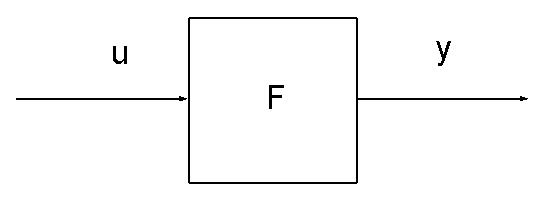
\includegraphics[width = 0.5\textwidth]{./Images/basic_block.eps}
	\caption{Illustration av ett enkelt blockschema.}
	\label{fig:basic_block}
\end{figure}

Med denna figuren menas att $Y(s) = F(s)U(s)$.

\paragraph{Rotort}
En rotort är en plott av ett systems poler som funktion av någon parameter. Den är typiskt uppdelad i grenar, som är kurvor i planet som är parametriserade av parametervärdet. Polerna som motsvarar parametervärdet $0$ är rotortens startpunkter, och polarna motsvarande parametervärdet $\infty$ är rotortens ändpunkter. Om rotorten närmar sig kurvor, är dessa rotortens asymptoter.

\section{Prestanda och prestandamått}

\paragraph{Stigtid}
Stigtiden definieras som $T_{\text{r}}, = t_{2} - t_{1}$, där vi typiskt har kriteriet $y(t_{2}) = 0.9$ och $y(t_{1}) = 0.1$, med $y$ mätt i relativa enheter.

\paragraph{Insvängningstid}
Insvängningstiden definieras som $\abs{y(t) - 1} < p$ när $t > T_{\text{s}}$, med $y$ mätt i relativa enheter. $p$ är typiskt lika med $0.05$.

\paragraph{Översläng}
Överslänget definieras som $y_{\text{max}} - 1$, med $y$ mätt i relativa enheter.

\paragraph{Parametrar i svängningslika system}
Om du har ett system med ett andra ordningens polynom i överförningsfunktionens nämnare, skriv polynomet som $s^{2} + 2\zeta\omega_{0}s + \omega_{0}^{2}$. $\omega_{0}$ är systemets resonansfrekvens och $\zeta$ dets dämpning. Det gäller för ett rent andra ordningens system att
\begin{align*}
	T_{\text{r}} \propto \frac{1}{\omega_{0}},\ T_{\text{s}} \approx \frac{3}{\zeta\omega_{0}},\ M = e^{\frac{\pi\zeta}{\sqrt{1 - \zeta^{2}}}}.
\end{align*}

\paragraph{Stationärt fel}
Det stationära felet är felet $e = r - y$ som kvarstår efter lång tid.

\paragraph{Felkoefficienter}
Det stationära felet beror både på systemets egenskaper och reglersignalen. Om reglersignalen är på formen $r_{n} = t^{n}\theta(t)$, där $\theta$ är Heavisidefunktionen, definieras felkoefficienterna som
\begin{align*}
	e_{n} = \lim\limits_{t\to\infty}r_{n} - y.
\end{align*}

\section{Blockschema}

\paragraph{Syftet med blockschema}
Blockschema är ett systematisk sätt att rita reglerade system på.

\paragraph{Hur funkar det?}
Betrakta blocket i figur \ref{fig:basic_block}.

\begin{figure}[!ht]
	\centering
	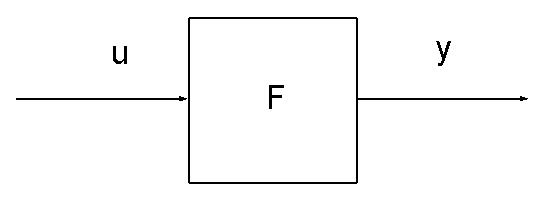
\includegraphics[width = 0.5\textwidth]{./Images/basic_block.eps}
	\caption{Illustration av ett enkelt block i ett blockschema.}
	\label{fig:basic_block}
\end{figure}

Med denna figuren menar vi exakt att $Y(s) = F(s)U(s)$.

\section{Negativ återkoppling}

\paragraph{Vad är negativ återkoppling?}
I denna kursen kommer vi att studera hur man kontrollerar ett system vid att låta avvikelsen mot det önskade värdet kontrollera regleringen av storheten.

\paragraph{Illustration i blockdiagram}
Ett enkelt negativt kontrollsystem illustrearas i figur \ref{fig:negative_feedback}.

\begin{figure}[!ht]
	\centering
	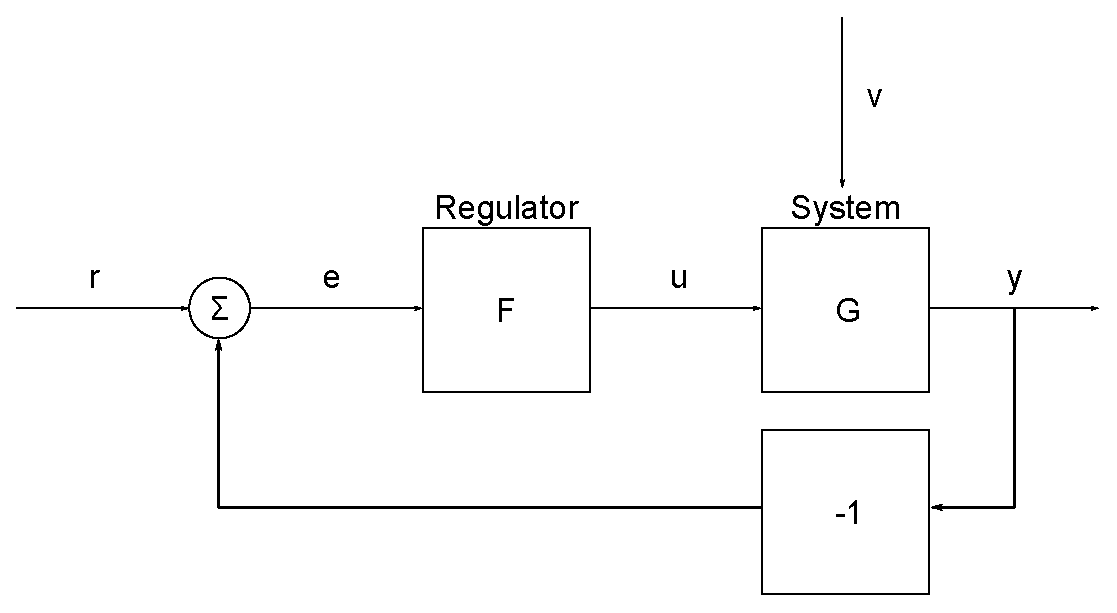
\includegraphics[width = \textwidth]{./Images/negative_feedback.eps}
	\caption{Schematisk illustration av ett enkelt negativt återkopplad system.}
	\label{fig:negative_feedback}
\end{figure}

\paragraph{Beskrivning av systemet}
Vi börjar beskrivningen av systemet med att inte betrakta störningar. I ena ändpunkten har vi
\begin{align*}
	Y = GU = GFE.
\end{align*}
Summationskomponenten till vänster ger oss
\begin{align*}
	E = R - Y,
\end{align*}
och därmed
\begin{align*}
	Y = GFR - GFY.
\end{align*}
Därmed kan vi skriva
\begin{align*}
	Y = \frac{GF}{1 + GF}R.
\end{align*}

\paragraph{Återkopplad överföringsfunktion}
För ett återkopplad system som kan skrivas som $Y = G_{\text{C}}R$ definieras $G_{\text{C}}$ som den återkopplade överföringsfunktionen. För systemet ovan har vi alltså
\begin{align*}
	G_{\text{C}} = \frac{GF}{1 + GF}R.
\end{align*}

\paragraph{Samband mellan reglerfel och referens}
Alternativt kan vi lösa systemet ovan för att få
\begin{align*}
	R - E = GFE,\ E = \frac{1}{1 + GF}R.
\end{align*}

\paragraph{Samband mellan referens och insignal}
Systemet ovan kan även lösas för att ge
\begin{align*}
	U = FR - FY = FR - GFU,\ U = \frac{F}{1  + GF}R.
\end{align*}

\paragraph{Slutna systems poler}
Vi ser att slutna system har poler där $1 + GF = 0$. Därmed bestäms systemets stabilitet av systemet och regulatorn.

\section{Frekvensanalys}

\paragraph{Fundamental ide}
Eftersom periodiska funktioner kan skrivas som en summa av trigonometriska funktioner och funktioner som avtar tillräcklig snabbt kan skrivas som en integral över trigonometriska funktioner, vet vi att när vi studerar linjära system räcker det att studera systemets respons på en enda term, alltså en enda trigonometrisk funktion, och se hur den beror av frekvensen. Om vi tillför en signal $u = \sin{\omega t}$ till ett system med överförningsfunktion $G$ får vi
\begin{align*}
	y &= \integ{0}{\infty}{\tau}{g(\tau)u(t - \tau)} \\
	  &= \Im\left(\integ{0}{\infty}{\tau}{g(\tau)e^{i\omega(t - \tau)}}\right) \\
	  &= \Im\left(e^{i\omega t}\integ{0}{\infty}{\tau}{g(\tau)e^{-i\omega\tau}}\right) \\
	  &= \Im(e^{i\omega t}G(i\omega)) \\
	  &= \abs{G(i\omega)}\sin(\omega t + \arg{G(i\omega)}).
\end{align*}
Det kan även finnas transienta termer här, men om systemet är stabilt kommer dessa försvinna över tid. Vi ser alltså att systemets svar beror av $G(i\omega)$.

\paragraph{Nyquistdiagram}
Ett Nyquistdiagram är en uppritning av $G(i\omega)$ för $0 < \omega < \infty$.

\paragraph{Bodediagram}
Ett Bodediagram är en uppritning av $\abs{G(i\omega)}$ och $\arg{G(i\omega)}$ som funktioner av $\omega$.

\paragraph{Bandbredd}
Bandbredden är bredden på det frekvensintervallet där $\abs{G(i\omega} \geq \frac{1}{\sqrt{2}}$, och benämnas $\omega_{\text{B}}$. Bandbredden kan ge information om systemets tillväxt, då hög bandbredd typiskt betyder snabb tillväxt. Man önskar typiskt att denna skall vara stor.

\paragraph{Resonansfrekvens}
Resonansfrekvensen $\omega_{\text{r}}$ är den frekvens som ger starkast respons i systemet.

\paragraph{Resonanstopp}
Resonanstoppen är $M_{\text{p}} = \abs{G(i\omega_{\text{r}})}$, och ger typiskt en indikation på hur mycket översläng man får. Man önskar typiskt att denna ska vara liten.

\paragraph{Stationärt fel}
Det stationära felet ges av $e_{0} = 1 - G_{\text{C}}(0)$.

\paragraph{Brytningspunkter}
Om överförningsfunktionen kan skrivas som
\begin{align*}
	G(i\omega) = \frac{\prod(i\omega - z_{i})}{\prod(i\omega - p_{i})},
\end{align*}
är alla $z_{i}$ och $p_{i}$ brytningspunkter för systemet. Här kommer de största lutningsändringarna i Bodediagrammet.

\paragraph{Bodes relation}
Låt $G$ vara minimumsfas, dvs. ha alla sina nollställen och poler i vänstre halvplan, och $G(0) > 0$. Då gäller att om $\abs{G(i\omega)}$ i ett visst frekvensområde avtar med \SI{20}{\deci\bel} per dekad (en dekad är en ökning i frekvens med en faktor $10$), är $\arg{G(i\omega)}\approx \SI{-90}{\degree}$, och om $\abs{G(i\omega)}$ avtar med \SI{40}{\deci\bel} per dekad, är $\arg{G(i\omega)}\approx \SI{-180}{\degree}$.

\paragraph{Snabbhet och svängighet}
Vi kan med tidigare resultat se att om $G_{\text{O}}(i\omega)$ är nära $1$ blir $G_{\text{C}}(i\omega)$ stor, och om $G_{\text{O}}(i\omega)$ är liten blir även $G_{\text{C}}(i\omega)$ liten. Vi kan också se att ett ekvivalent kriterium för bandbredden är $\abs{G_{\text{O}}(i\omega) - 1} \leq \sqrt{2}$ för $\omega \geq \omega_{\text{B}}$.

\paragraph{Resonanstopp och fasmarginal}
Vi har
\begin{align*}
	M_{\text{p}} \geq \abs{G(i\omega_{\text{c}})} = \frac{1}{2\sin(\frac{1}{2}\phi_{\text{m}})}.
\end{align*}
Speciellt ger liten fasmarginal stort översläng.

\section{Kompensering}

\paragraph{Ideen}
Vi ser att det enklaste sättet att konstruera en bra regulator på är att ändra konstruktionen av det öppna systemet. Vi bestämmer alltså regulatorn $F$ utifrån krav på
\begin{itemize}
	\item snabbhet, alltså skärfrekvens.
	\item dämpning, alltså fasmarginal.
	\item stationärt fel, alltså krav på $\abs{G_{\text{O}}(0)}$.
\end{itemize}

\paragraph{Kompensation för snabbhet}
För snabbhet räcker det med en P-regulator. Denna flyttar amplitudkurvan, men ändrar ej faskurvan. Alltså hjälper den oss att bestämma skärfrekvensen.

\paragraph{Dämpning}
Här kan man använda en PD-regulator. Den fixar fasmarginalen.

\paragraph{Stationärt fel}
Här kan man använda en PI-regulator. Denna kan dock förstöra fasmarginalen.

\paragraph{Arbetsgång}
Arbetsgången i kompensering är att
\begin{itemize}
	\item bestämma önskad bandbredd.
	\item bestämma önskad fasmarginal för att ge nödvändig fasökning vid skärfrekvensen.
	\item Gör lead- och laggrejer. Jag kanske borde fatta det.
\end{itemize}

\section{Tillståndsrepresentationer}

\paragraph{Ideen}
Den fundamentala ideen vi vill åt nu är att representera ett systems tillstånd på ett annat sätt än just dets tidsutveckling, till exempel som en vektor.

\paragraph{Representation av linjära system}
Tidsutvecklingen av ett system tillstånd kan i många linjära fall skrivas som
\begin{align*}
	\dot{x} = Ax + Bu,
\end{align*}
där $u$ beskriver en styrsignal. Utsignalen är typiskt på formen
\begin{align*}
	y = Cx + Du.
\end{align*}

\paragraph{Linjära system i Laplacedomänet}
Genom att laplacetransformera ekvationen som beskriver ett systems tillstånd fås
\begin{align*}
	sX = AX + BU,
\end{align*}
givet att systemets starttillstånd är $\vb{0}$. Detta kan skrivas som
\begin{align*}
	X = (sI - A)^{-1}BU.
\end{align*}
Insatt i uttrycket för $Y$ fås
\begin{align*}
	Y = CX + DU = (C(sI - A)^{-1}B + D)U,
\end{align*}
och vi identifierar överförningsfunktionen som
\begin{align*}
	G = C(sI - A)^{-1}B + D.
\end{align*}
Av någon anledning är detta lika med
\begin{align*}
	G = \frac{1}{sI - A}C(sI - A)^{\dagger}B + D
\end{align*}

\paragraph{Poler i tillståndsrepresentation}
Det visar sig att systemets poler ges av
\begin{align*}
	\det(sI - A) = s^{2}.
\end{align*}
Detta ska tydligen motsvara $A$:s egenvärden.

\paragraph{Linjarisering}
Verkliga system är ofta olinjära, men vi ska försöka behandla dem som linjära ändå.

Betrakta ett system
\begin{align*}
	\dot{x} = f(x, u),\ \dot{y} = g(x, u).
\end{align*}
Anta konstant styrsignal $u_{0}$, och antag att systemet då tenderar mot ett stationärt tillstånd $\vb{x}_{0}$. Denna punkten uppfyller då
\begin{align*}
	f(x_{0}, u_{0}) = \vb{0},\ h(x_{0}, u_{0}) = y_{0}.
\end{align*}
När vi linjäriserar, betraktar vi små variationer $\Delta x, \Delta u, \Delta y$ kring denna punkten. Vi får
\begin{align*}
	\dv{\Delta x}{t} = f(x_{0} + \Delta x, u_{0} + \Delta u) = \vb{f}(x_{0}, u_{0}) + \pdv{f}{x}\Delta x + \del{u}{f}\Delta u = \pdv{f}{x}\Delta x + \del{u}{f}\Delta u.
\end{align*}
Observera att $\pdv{f}{x}$ allmänt är en matris.

På samma sätt fås
\begin{align*}
	\dv{\Delta y}{t} = h(x_{0} + \Delta x, u_{0} + \Delta u) - y_{0} = h(x_{0}, u_{0}) - y_{0} + \grad_{x}{h}\Delta x + \del{u}{h}\Delta u = \grad_{x}{h}\Delta x + \del{u}{h}\Delta u.
\end{align*}
Det totala systemet
\begin{align*}
	\dv{\Delta x}{t} &= \pdv{f}{x}\Delta x + \del{u}{f}\Delta u, \\
	\dv{\Delta y}{t}     &= \grad_{x}{h}\Delta x + \del{u}{h}\Delta u
\end{align*}
är alltså linjärt för små ändringar.

\paragraph{Lösning av system i representation}
Betrakta ett system på formen
\begin{align*}
	\dot{\vb{x}} = A\vb{x} + Bu,\ \vb{x}(0) = \vb{x}_{0},\ y = C\vb{x}.
\end{align*}
Vi använder att
\begin{align*}
	\dv{t}e^{-At} = -Ae^{-At},
\end{align*}
varför
\begin{align*}
	e^{-At}\dot{\vb{x}}              &= e^{-At}A\vb{x} + e^{-At}Bu, \\
	\dv{t}\left(e^{-At}\vb{x}\right) &= e^{-At}Bu, \\
	\vb{x}                           &= \vb{x}_{0}e^{At} + \integ{0}{t}{\tau}{e^{-A(t - \tau)}Bu}.
\end{align*}

\paragraph{Styrbarhet}
Ett tillstånd $\vb{x}$ är styrbart om man kan styra det motsvarande systemet från $\vb{0}$ till $\vb{x}$ med hjälp av en styrsignal $u$ på ändlig tid.

\paragraph{Test av styrbarhet}
Vi noterar först att Cayley-Hamiltons sats ger
\begin{align*}
	A^{n} + \sum\limits_{i = 1}^{n}a_{i}A^{n - i} = 0,
\end{align*}
där $a_{i}$ är koefficienterna i $A$:s karakteristiska polynom. Därmed kan alla potenser av $A$ av högre ordning skrivas som en linjärkombination av potenser av $A$ upp till och med $n - 1$. Därmed gäller det att
\begin{align*}
	e^{At} = \sum\limits_{i = 0}^{n - 1}f_{i}(t)A^{i}
\end{align*}
för några funktioner $f_{i}$.

Betrakta nu ett system och dets representation. Om systemets starttillstånd är $\vb{0}$, medför detta
\begin{align*}
	\vb{x} = \left(\sum\limits_{i = 0}^{n - 1}\gamma_{i}(t)A^{i}\right)\vb{b}
\end{align*}
där
\begin{align*}
	\gamma_{i} = \integ{0}{t}{\tau}{f_{i}(\tau)u(\tau)}.
\end{align*}
Med andra ord är de styrbara $\vb{x}$ linjärkombinationer av de olika $A^{i}\vb{b}$, alltså att det ligger i bildrummet till styrbarhetsmatrisen
\begin{align*}
	\S = [\vb{b}, A\vb{b}, \dots, A^{n - 1}\vb{b}].
\end{align*}
Systemet är styrbart om $\det(\S) \neq 0$.

\paragraph{Observerbarhet}
Ett tillstånd $\vb{x}$ är icke observerbart om utsignalen $y$ är identiskt noll då initialvärdet är $\vb{x}$ och insignalen identisk noll.

\paragraph{Test av observerbarhet}
Vi vill nu testa om ett tillstånd $\vb{x}_{0}$ är observerbart. Om vi har styrsignal $u = 0$, gäller det att
\begin{align*}
	\vb{x} = e^{At}\vb{x}_{0}, y = \vb{c}\cdot e^{At}\vb{x}_{0}, \dv[n]{y}{t} = \vb{c}\cdot A^{n}e^{At}\vb{x}_{0}.
\end{align*}
Speciellt är $y = 0$ för alla $t$ om
\begin{align*}
	y(0) = \vb{c}\cdot\vb{x}_{0} = 0, \dv{y}{t} = \vb{c}\cdot A\vb{x}_{0} = 0,\ \dots, \dv[n - 1]{y}{t} = \vb{c}\cdot A^{n - 1}\vb{x}_{0} = 0.
\end{align*}
Givet att detta stämmer, ger Cayley-Hamiltons sats att även högre ordningens derivator av $y$ kommer vara $0$. Därmed ligger de icke-observerbara tillstånden i nollrummet till observerbarhetsmatrisen
\begin{align*}
	\O =
	\mqty[
		\vb{c}^{T} \\
		\vb{c}^{T}A \\
		\vdots \\
		\vb{c}^{T}A^{n - 1}
	].
\end{align*}
Systemet är observerbart $\det(\O) \neq 0$.

\paragraph{Minimalhet}
Ett system är minimalt om och endast om det är både styrbart och observerbart.

\paragraph{Proportionell återkoppling}
Antag att vi återkopplar systemet med $\vb{u} = l_{0}\vb{r} - L\vb{x}$. Om utsignalen ej beror av $\vb{u}$ kan det återkopplade systemet skrivas som
\begin{align*}
	\dot{\vb{x}} = (A - BL)\vb{x} + Bl_{0}\vb{r},\ y = C\vb{x}.
\end{align*}

Systemets poler ges av egenvärdena till $A - BL$. Det finns $n$ såna, och $L$ har $n$ parametrar. Om systemet är styrbart kan dets poler därmed placeras godtyckligt vid lämpligt val av $L$.

Valet av $l_{0}$ görs så att $y = r$ när systemet är stationärt. Detta kräver dock att man känner $G(0)$ och att inga störningar påverkar systemet. Därför inför vi I-reglering.

\paragraph{I-reglering}
När vi I-reglerar, inför vi extra tillstånd
\begin{align*}
	x_{n + 1} = \integ{0}{t}{\tau}{e}.
\end{align*}
Detta ger
\begin{align*}
	\dot{x}_{n + 1} = r - y = r - Cx.
\end{align*}
Då kan vi utvidga modellen till
\begin{align*}
	\dot{\vb{x}} =
	\mqty[
		\dot{x} \\
		\dot{x}_{n + 1}
	]
	=
	\mqty[
		A  & 0 \\
		-C & 0
	]
	\mqty[
		x \\
		x_{n + 1}
	] +
	\mqty[
		B \\
		0
	]
	u
	+
	\mqty[
		0 \\
		1
	]
	r = A\vb{x} + Bu + 
	\mqty[
		0 \\
		1
	]
	r.
\end{align*}
Strategin är nu att återkoppla det nya systemet med återkoppling på formen
\begin{align*}
	u = -Lx - l_{n + 1}x_{n + 1} = -L\vb{x}.
\end{align*}
Då kan $L$ väljas så att $A - BL$ får önskade egenvärden. Stationärt har vi
\begin{align*}
	\dot{x} = 0,\ 	\dot{x}_{n + 1} = 0.
\end{align*}

\paragraph{Skattning av tillstånd}
Om man ej kan mäta systemets tillstånd exakt, kan man skatta det.

Mer precist, antag att vi har en modell
\begin{align*}
	\dot{x} = Ax + Bu,\ y = Cx
\end{align*}
som simulerar
\begin{align*}
	\dot{\hat{x}} = A\hat{x} + Bu,\  \hat{y} = C\hat{x}.
\end{align*}
Felsignalen är
\begin{align*}
	y - \hat{y} = y - C\hat{x}.
\end{align*}
Vi försöker återkoppla systemet. Det beskrivs då av
\begin{align*}
	\dot{\hat{x}} = A\hat{x} + Bu + K(y- C\hat{x}) = (A - KC)C\hat{x} + Bu + Ky.
\end{align*}
Skattningsfelet $\tilde{x}$ ges då av
\begin{align*}
	\dot{\tilde{x}} = \dot{x} - \dot{\hat{x}} = Ax + Bu - A\hat{x} - Bu - K(Cx - C\hat{x}) = (A - KC)\tilde{x}.
\end{align*}
Detta har lösning
\begin{align*}
	\tilde{x} = e^{(A - KC)t}\tilde{x}(0).
\end{align*}
Felet tenderar mot $0$ egenvärdena till $A - KC$ är negativa, och hur snabbt det tenderar mot $0$ beror av egenvärdenas belopp.

Mätfelet ges av $y_{\text{m}} = y + e$. Detta ger
\begin{align*}
	\dot{\tilde{x}} = (A - KC)\tilde{x} + Ke.
\end{align*}
Stora $K$ ger som vi ser höga mätfel, men det ger även snabba system. Optimeringen där görs av ett Kalmanfilter. Vi väljer då systemet så att egenvärdena till $A - BL$ har lägre belopp än egenvärdena till $A - KC$.

Vid återkoppling av såna system är överförningsfunktionen för det slutna systemet
\begin{align*}
	G = C(sI - (A - BL))^{-1}Bl_{0},
\end{align*}
alltså likadant som tidigare.

\end{document}
